%% ID: hinged_rod
%% TITLE: A hinged rod
%% TYPE: question
%% QUESTIONTYPE:  numerical
%% CONCEPTS: forces, friction, newtoni
%% VIDEOS: 
%% LEVEL: 4
%% TOPIC: mechanics/statics
%% ORDER: 10

\begin{problem}[A1987MsQ10p]%beams, hinges, friction
{\exposition{A uniform rod of length \vari{2a} runs from A to B and has mass \vari{km}. The rod is hinged at both ends with the point A fixed. The other end is freely hinged to another rod of length \vari{2a} and mass \vari{m}. Both rods are in equilibrium with the first rod horizontal and the second is inclined at some angle \vari{\theta} to the vertical with its unhinged end in contact with the rough floor. The coefficient of friction between the rod and the floor is \vari{\mu}. See Figure \ref{fig:Statics_Hinged_Rods_1}.}
\question{Show that
	\begin{equation*}
	\mu\ge \frac{1+k}{2+k}\tan(\theta)	
	\end{equation*}}
	
\begin{figure}[h]
	\centering
	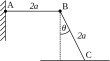
\includegraphics[width=0.4\textwidth]{../../../figures/Statics_Hinged_Rods_1.svg}
	\caption{}	
	\label{fig:Statics_Hinged_Rods_1}
\end{figure}
	
}
{\textit{Used, with permission from UCLES, A Level Maths, Syllabus A, June 1987, Special Paper, Question 10.}}
{\answer{}
This question requires us to think about the forces on $each$ rod, paying particular attention to the forces at the hinges. See Figure \ref{fig:Statics_Hinged_Rods_2} for all the forces acting on each rod, which will allow us to take moments. Remember that at a hinge (or pin joint) there is no resultant force for the system, however there are equal and opposite forces acting on each rod in both the vertical and horizontal directions. 

\begin{figure}[h]
	\centering
	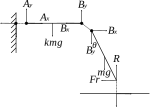
\includegraphics[width=0.5\textwidth]{Statics_Hinged_Rods_2}
	\caption{}	
	\label{fig:Statics_Hinged_Rods_2}
\end{figure}

However, we can first resolve vertically for the whole system (ignoring the joint at B):

\begin{align*} A_y + R = mg(k+1) \end{align*}

Also, resolve vertically just for rod AB:

\begin{align*} A_y + B_y = kmg \end{align*}

Moments about A for AB:

\begin{align*} kmga = 2B_{y}a \\
B_y = \frac{kmg}{2} \end{align*}

Moments about C for BC:

\begin{align*} amg\sin(\theta) + 2aB_{y}\sin(\theta) = 2aB_{x}\cos(\theta)\end{align*}

Finally, resolve horizontally for BC:

\begin{align*} Fr = B_x = \mu R \end{align*}

Now all we need to do is solve these simultaneous equations:

\begin{align*} A_y &= mg(k+1) -R\\
kmg - B_y &= mg(k+1)-R \\
kmg - \frac{kmg}{2} &= mg(k+1) -R \\
R &= mg\left(\frac{k}{2} + 1\right) \\
\intertext{Hence} B_x = \mu mg\left(\frac{k}{2} + 1\right)\end{align*}

Now sub $B_x$ and $B_y$ into the moments about C equation, and solve for $\mu$:

\begin{align*}mg\sin(\theta) + kmg\sin(\theta) &= 2\mu mg\left(\frac{k}{2} + 1\right)\cos(\theta) \\
\\ \tan(\theta)(1+k) &= \mu (k+2) \\
\\ \mu &= \tan(\theta) \frac{1+k}{2+k}\end{align*}

Remember, this is limiting equilibrium. For values of $\mu$ less than this the system will not be in equilibrium. Hence:

\begin{align*} \mu \ge  \frac{1+k}{2+k}\tan(\theta) \end{align*}

As required


}
\end{problem}